\documentclass[runningheads]{llncs}
\usepackage[T1]{fontenc}
\usepackage{amsmath}
\usepackage[usenames, dvipsnames]{xcolor}
\usepackage{pgfplots}
\usetikzlibrary{calc, positioning, shapes.geometric}
\pgfplotsset{compat=newest}

\begin{document}

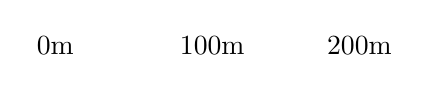
\begin{tikzpicture}
    \node[] (black) {0m};
    \node[right=1.1cm of black] (pink) {100m};
    \node[right=0.8cm of pink] (yellow) {200m};
  \end{tikzpicture}

\end{document}